\section*{Exercice 2 : Binary buddy system (3 points)}

Un consid�re un allocateur de m�moire grain-fin de type \emph{malloc}
bas� sur un buddy system binaire d'ordre 12 (qui peut allouer des blocs
d'une taille maximale de 2$^{12}$ octets).

L'allocateur dispose initialement d'un bloc libre de 4 ko.

Le programme effectue successivement des appels � \emph{malloc} avec
les tailles suivantes : 126, 510, 1200, 10, 1000 et 498 octets.

\begin{enumerate}
\item Donnez l'�tat de l'allocateur, c'est-�-dire l'ensemble des blocs
libres et occup�s apr�s chacune de ces allocations.

\begin{correction}

Allocation de 126 octets.

  \begin{center}
    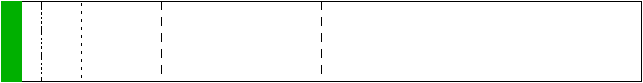
\includegraphics[width=0.5\linewidth]{figures/buddy-1}
  \end{center}

Allocation de 510 octets.

  \begin{center}
    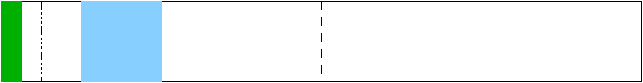
\includegraphics[width=0.5\linewidth]{figures/buddy-2}
  \end{center}

Allocation de 1200 octets.

  \begin{center}
    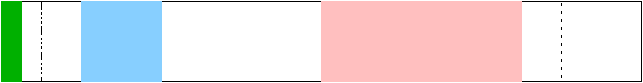
\includegraphics[width=0.5\linewidth]{figures/buddy-3}
  \end{center}

Allocation de 10 octets.

  \begin{center}
    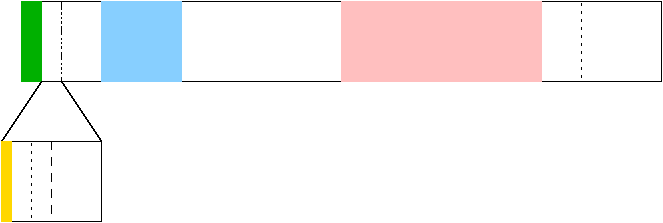
\includegraphics[width=0.5\linewidth]{figures/buddy-4}
  \end{center}

Allocation de 1000 octets.

  \begin{center}
    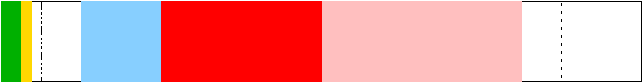
\includegraphics[width=0.5\linewidth]{figures/buddy-5}
  \end{center}

Allocation de 498 octets.

  \begin{center}
    
\includegraphics[width=0.5\linewidth]{figures/buddy-6}
  \end{center}

\end{correction}

\item Calculez le taux de fragmentation de la m\'emoire apr\'es ces 6
allocations.

\begin{correction}

Taille totale allou�e (utilisateur) : $126+510+1200+10+1000+498 = 3344$\\
Taille totale allou�e (r�el) : $128+512+1280+16+1024+512 = 3472$\\
Taux de fragmentation : $1 - \frac{3344}{3472} = 3.7 \%$

\end{correction}

\item On veut maintenant allouer un bloc de 2000 octets.
Que se passe-t-il lors cette derni�re allocation ? Que pr�conisez-vous ?

\begin{correction}

Il n'y a aucun bloc d'au moins 2000 octets disponible. L'allocateur
doit demander une nouvelle page au noyau. Il divisera alors cette page
en deux bloc de 2 ko chacun, et retournera l'un d'eux � l'utilisateur.

\end{correction}

\end{enumerate}
